\documentclass[]{report}
\usepackage{bookmark}
\usepackage[utf8]{inputenc}
\usepackage{authblk}
\usepackage{amsmath,amsfonts,amsthm,amssymb,mathtools}
\usepackage[english]{babel}


%% theorem, lemma, proof, etc. %%
%% for unnumbed use \newtheorem* and delete section in [---] %%
\newtheorem{theorem}{Theorem}[section]
\newtheorem{corollary}{Corollary}[theorem]
\newtheorem{lemma}[theorem]{Lemma}
\newtheorem{proposition}[theorem]{Proposition}

\theoremstyle{remark}
\newtheorem{remark}{Remark}

\theoremstyle{definition}
\newtheorem{definition}{Definition}[section]

\theoremstyle{definition}
\newtheorem{example}{Example}[section]
%%% theorem %%

\usepackage{enumitem}
\usepackage{graphicx}
\usepackage{tikz}
\usetikzlibrary{decorations.fractals}
\usepackage{float}
\usepackage{dsfont}
\usepackage{geometry}
\geometry{
    a4paper,
    %%% left=30mm,
    %%% right=30mm,
    %%% top=20mm,
    %%% bottom=20mm,
}

%%%% hyperref %%%%
\usepackage{hyperref} % for link
\hypersetup{
    colorlinks=true,
    allcolors=black,
}
%%% fancyhdr %%%% for footer and Hader of document
\usepackage{fancyhdr}
\usepackage{cleveref}
%\pagestyle{fancy}
%\lhead{lest hand head} %% left Hader %%
%\rhead{Measure Theory} %% right Hader %%
\cfoot{\thepage} %% central footer %%

\setlength{\headheight}{14.49998pt}

%%% spacing in document %%%
\usepackage{setspace}
\onehalfspacing

\title{Markov Chain}
\author{Azmain Biswas}
\date{April 2023}

\begin{document}

\maketitle
\tableofcontents

\chapter{Introduction}
The Weak law of large number(WLLN) and the Central Limit theorem(CTL) proved around  1880's. At that time those were the focal probabilistic issues.
In 1902 Russian Mathematician cum Philosopher P.A. Nekrasov claimed that pairwise independent of random variables were necessary condition for CTL to hold. 
This motivated Andrei A. Markov to construct a counterexample to disprove the claim of P.A. Nekrasov. So He developed Markov Chain in 1907 to disprove a 
"Mathematical proof of freewill" which had been proposed by P.A.Nekrasov to defend the church.

 A Markov chain is a stochastic model that describes a sequence of possible
events or transitions from one state to another of a system. The probability of transitions
from state to state only depends on the current state of the system. A Markov Chain is
used to unravel predictions about future states of a stochastic process using only knowledge
of the present state. This property of “forgetting” past states is known as the memoryless
property.

Now a days Markov Chain is a very important concept, it is used in various fields like computer science, mathematics, physics, economics, and more.
Markov chains have proven to be an effective modelling and analysis method for systems that change over time.


\chapter{Markov Chain}

\section{Definition}

\begin{definition}[Markov Chain]
    A discrete time stochastic process $\{X_n,n=1,2,3,\ldots\}$ is defined to be \textit{Discrete Time Markov Chain} or simply \textit{Markov Chain}
    if it takes value  the state space $ \mathbf{S} $, and for every
    $n\ge 0$ it satisfy the property
    \begin{equation}
        \label{Markov property}
         \mathbf{P}( X_{n+1} = j | X_n =i , X_{n-1} = i_{n-1}, \ldots, X_0 = i_0 ) = \mathbf{P}( X_{n+1} = j | X_n =i )
    \end{equation}
\end{definition}

Unless otherwise mentioned we take the state space $ \mathbf{S} $ to be $\{0, 1, 2, 3, \ldots\ \} $. 
If $X_n = i $ we say that the process is in $i $th state at time $n$.
In the definition \cref{Markov property} may be interpreted as for Markov Chain, the conditional distribution of any future state $ X_{n+1} $, given the past states  $ X_0, X_1,\ldots, X_{n-1} $  and the present state $ X_n $, is independent of the past and only depend on the present state.
This property is called \textit{Markovian Property}. In other word for Markov chain predicting the future we only need information about the present state.

\textbf{Note:} Assumption we are making for Markov chain to forget the past as long as present in known is very strong assumption.

\section{Homogeneous Markov Chain}

\begin{definition}[Homogeneous Markov Chain]
    We say a Markov chain $ \{ X_n,n\ge 0 \} $ is homogeneous if $ \mathbf{P}(X_{n+1}=j|X_n=i)=\mathbf{P}(X_2=j|X_1=i) \ \forall n>0 $. 
\end{definition}

The quantity $ \mathbf{P}(X_{n+1}=j|X_n=i) $ is called the \textit{transition probability} from state $i$ to state $j$. For homogeneous Markov Chain 
we can specify the transition probabilities $ \mathbf{P}(X_{n+1}=j|X_{n}=i) $ by a sequence of value $ p_{ij} = \mathbf{P}(X_{n+1}=j|X_{n}=i) $.

Then the transition probabilities are $ p_{ij}, $ 
$ 1\le i,j \le \infty $ for transition from state i to state j. The matrix  $ P = (p_{ij}) $ is called The
\textit{Transition Matrix} of chain. Since probabilities are nonnegative and since the process must make a transition into some state, we have
\[
    p_{ij}\ge 0,\ \ i,j\ge 0,\ \text{and } \sum_{j=0}^{\infty}p_{ij} = 1,\ \  \forall\ i=0,1,2,\ldots.
\]

For, infinite state Markov chain the probability transition matrix will be infinite order. 
Then,
\[
    P = 
    \begin{bmatrix}
        p_{00} & p_{01} & p_{02} & \ldots \\
        p_{10} & P_{11} & p_{12} & \ldots \\
        \vdots & \vdots & \vdots & \ldots \\ 
        p_{i0} & \ldots & p_{ij} & \ldots \\
        \vdots & \vdots & \vdots & \ddots 
    \end{bmatrix}
\]

\begin{example}[Rain and sunny]
    Suppose that whether it rains today depends on previous weather conditions only from the last two days. 
    Specifically, suppose that if it has rained for the past two days, 
    then it will rain tomorrow with probability 0.7; 
    if it rained today but not yesterday, then it will rain tomorrow with probability 0.5; 
    if it rained yesterday but not today, then it will rain tomorrow with probability 0.4; 
    if it has not rained in the past two days, then it will rain tomorrow with probability 0.2.
    
    We can transform it into a Markov chain by letting the state on any day be determined by the weather conditions during both that day and 
    the preceding one. For instance, we can say that the process is in

    \begin{center}
        State 0: if it rained both today and yesterday\\ 
        State 1: if it rained today but not yesterday\\ 
        State 2: if it rained yesterday but not today\\ 
        State 3: if it rained neither today nor yesterday 

    \end{center}

    The it will be 4-state Markov chain whose transition matrix will be,
    \[
        P=
        \begin{bmatrix} 
            0.7 & 0 & 0.3 & 0 \\ 
            0.5 & 0 & 0.5 & 0 \\ 
            0 & 0.4 & 0 & 0.6 \\ 
            0 & 0.2 & 0 & 0.8
        \end{bmatrix} 
    \]
\end{example}

\section{Chapman-Kolmogorov Equations}
We have already defined the one step transition probabilities $ p_{ij} $. We now define the n-step transition probabilities $ p_{ij}^{n} $ 
to be the probability that a process in state $i$ will be in state $j$ after $n$ additional transitions. i.e.
\[
    p^{n}_{ij}=\mathbf{P}(X_{n+m}=j|X_{m}=i), \ n\ge 0, \ i,j\ge 0.
\]

By definition of Markov chain we get,
\begin{align*}
    p_{ij}^{n+m} &= \mathbf{P}(X_{n+m}=j|X_{0}=i) \\ 
                 &= \sum_{k=0}^{\infty}\mathbf{P}(X_{n+m}=j,X_{n}=k|X_{0} = i)\text{ (By theorem of total probability)} \\
                 &= \sum_{k=0}^{\infty}\mathbf{P}(X_{n+m}=j|X_{n}=k,X_{0} = i)\mathbf{P}(X_{n}=k|X_{0}=i) \\
                 &= \sum_{k=0}^{\infty}\mathbf{P}(X_{n+m}=j|X_{n}=k)\mathbf{P}(X_{n}=k|X_{0}=i) \\
\end{align*}
Then,
\begin{align*}
     p_{ij}^{n+m} = \sum_{k=0}^{\infty}p_{kj}^{m}p_{ik}^{n}. \numberthis \label{Chapman-Kolmogorov equation} \\
\end{align*}
If we take $ n=m=1 $. Then
\begin{equation}
    \label{2-step probability}
    p_{ij}^{2} = \sum_{k=0}^{\infty} p_{kj}p_{ik}
\end{equation}
the above expression is $ (i,j) $ element of $ P^{2} $ matrix then we see \cref{2-step probability} in matrix form,
\[
    P^{2}=P\cdot P
\]
Hence, \cref{Chapman-Kolmogorov equation} can also written in matrix form,
\[
    P^{n+m}=P^{n}\cdot P^{m}
\]
Where $ P^{n}\ \text{ and } P^{m} $ are the $n$-step and $m$-step transition matrix respectively.

\begin{example}[Transition matrix of 4-state Markov chain]
    Consider the 4-state
    Markov chain depicted in Fig \ref{4-step transition matrix example} When no probabilities are written over the
    arrows, as in this case, it means all arrows originating from a given state are equally
    likely. For example, there are 3 arrows originating from state 1, so the transitions
    $1 \to 3$, $1 \to 2$, and $1 \to 1$ all have probability 1/3. Therefore, the transition matrix of the chain is.

    \begin{figure}[ht]
        \centering
        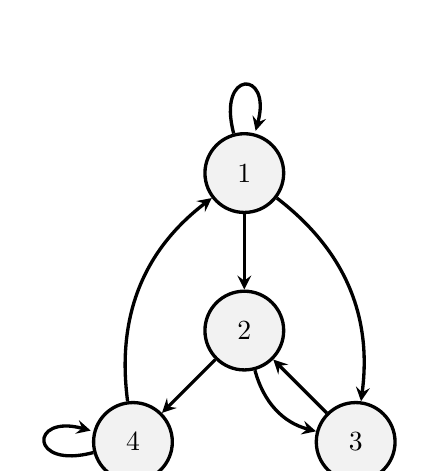
\begin{tikzpicture}[->, >=stealth, auto, very thick, node distance = 2cm, state/.style={circle, draw=black, fill=black!5, very thick, minimum size = 10mm}]
            \node[state] (1) {$1$};
            \node[state] (2) [below of=1] {$2$};
            \node[state] (3) [below right of=2] {$3$};
            \node[state] (4) [below left of=2] {$4$};

            \path (1) edge [loop above] (1)
                (1) edge []  (2)
                (1) edge [bend left] (3)
                (2) edge [bend right] (3)
                (2) edge [] (4)
                (3) edge [] (2)
                (4) edge [bend left] (1)
                (4) edge [loop left] (4);
        \end{tikzpicture}
        \caption{Example of a 4-state Markov chain}
        \label{4-step transition matrix example}
    \end{figure}

    \[
        P=
        \begin{bmatrix}
            \frac{1}{3} & \frac{1}{3} & \frac{1}{3} & 0 \\
            0 & 0 & \frac{1}{2} & \frac{1}{2} \\ 
            0 & 1 & 0 & 0 \\ 
            \frac{1}{2} & 0 & 0 & \frac{1}{2} 
        \end{bmatrix}
    \]
    To compute the probability that the chain is in state 3 after 5 steps, starting at
    state 1, we would look at the (1,3) entry of $ P^{5} $.
    \[
        P^5 =
        \begin{bmatrix}
            \frac{853}{3888} & \frac{509}{1944} & \frac{52}{243} & \frac{395}{1296} \\
            \frac{173}{864} & \frac{85}{432} & \frac{31}{108} & \frac{91}{288} \\
            \frac{37}{144} & \frac{29}{72} & \frac{1}{9} & \frac{11}{48} \\
            \frac{499}{2592} & \frac{395}{1296} & \frac{71}{324} & \frac{245}{864} \\
        \end{bmatrix}
    \]
    so, $ p^{5}_{13}=\mathbf{P}(X_{5}=3|X_{0}=1) = \frac{52}{243} $.
\end{example}

To get the marginal distributions of $X_0, X_1,...$ , we need to specify not just the
transition matrix, but also the initial conditions of the chain. This can be done by
setting the initial state $X_{0}$ to be a particular state, or by randomly choosing $X_0$
according to some distribution. Let $(t_1, t_2,...,t_N)$ be the PMF of $X_{0}$ displayed as
a vector, that is, $t_i = \mathbf{P}(X_0 = i)$. Then the marginal distribution of the chain at any time can be computed from the transition matrix.

\begin{proposition}[Marginal Distribution of $ X_{n} $]
    Define $ \mathbf{t} = (t_{1}, t_{2}, \ldots, t_{n})$ by $ t_{i}=\mathbf{P}(X_{0}=i) $, and view $ \mathbf{t} $ as a row vector.
    Then the marginal distribution of $ X_{n} $ is given by the vector $ \mathbf{t}P^{n} $. That is the $ j $-th component of  $ \mathbf{t}P^{n} $ 
    is $ \mathbf{P}(X_{n}=j) $.
\end{proposition}
\begin{proof}
    By the law of total probability we get,

    \begin{align*}
        \mathbf{P}(X_{n}=j) &= \sum_{i=0}^{N} \mathbf{P}(X_{n},X_{0}=i)\\
                            &= \sum_{i=0}^{N} \mathbf{P}(X_{0}=i)\mathbf{P}(X_{n}=j|X_{0}=i)
    \end{align*}

    \begin{equation*}
                                    = \sum_{i=0}^{N} t_{i}p^{n}_{ij}
    \end{equation*}
    Which is the $ j $-th component of  $ \mathbf{t}P^{n} $.
\end{proof}

\begin{example}[Marginal distribution of 4-state Markov chain]
    Again consider the 4-state Markov chain in Fig. \ref{4-step transition matrix example}. 
    Suppose the initial conditions are $ \mathbf{t} = (1/4,1/4,1/4,1/4) $, Let $ X_{n} $ be the position of the chain at time $ n $. 
    Then distribution of  $ X_{1} $ is
    \begin{align*}
        \mathbf{t}P &= \begin{bmatrix} \frac{1}{4} & \frac{1}{4} & \frac{1}{4} & \frac{1}{4} \end{bmatrix} 
        \begin{bmatrix}
            \frac{1}{3} & \frac{1}{3} & \frac{1}{3} & 0 \\
            0 & 0 & \frac{1}{2} & \frac{1}{2} \\ 
            0 & 1 & 0 & 0 \\ 
            \frac{1}{2} & 0 & 0 & \frac{1}{2} 
        \end{bmatrix}\\
                    &= \begin{bmatrix} \frac{5}{24} & \frac{1}{3} & \frac{5}{24} & \frac{1}{4} \end{bmatrix} 
    \end{align*}
    The marginal distribution of $ X_{5} $ is 
    \begin{align*}
        \mathbf{t}P^{5} &= \begin{bmatrix} \frac{1}{4} & \frac{1}{4} & \frac{1}{4} & \frac{1}{4} \end{bmatrix}
        \begin{bmatrix}
            \frac{853}{3888} & \frac{509}{1944} & \frac{52}{243} & \frac{395}{1296} \\
            \frac{173}{864} & \frac{85}{432} & \frac{31}{108} & \frac{91}{288} \\
            \frac{37}{144} & \frac{29}{72} & \frac{1}{9} & \frac{11}{48} \\
            \frac{499}{2592} & \frac{395}{1296} & \frac{71}{324} & \frac{245}{864} \\
        \end{bmatrix}\\
                        &= \begin{bmatrix}
                            \frac{707}{3254} & \frac{472}{1619} & \frac{101}{486} & \frac{1469}{5184}
                        \end{bmatrix} \\
    \end{align*}
\end{example}


\end{document}
